\begin{frame}[fragile]{Efficient, correct, safe, and secure}
\begin{minipage}{0.55\linewidth}
  \lstset{
    language=Jasmin,
    basicstyle=\footnotesize\ttfamily,
    escapechar=~~,
  }
  \begin{lstlisting}
fn memeq(reg u64 p q n) -> reg u64 {~~\loc{a00}~~
  reg u64 r one i;~~\loc{a01}~~
  r = 0;~~\loc{a02}~~
  one = 1;~~\loc{a03}~~
  i = 0;~~\loc{a04}~~
  while (i < n) {~~\loc{a05}~~
    if (r != 0) {~~\loc{a06}~~
      reg u64 a b;
      a = [p];~~\loc{a07}~~
      b = [q];~~\loc{a08}~~
      r = a != b ? one : r;~~\loc{a09}~~
      p += 8;~~\loc{a10}~~
      q += 8;~~\loc{a11}~~
    }~~\loc{a12}~~
    i = #INC(i);~~\loc{a13}~~
  }~~\loc{a14}~~
  return r;~~\loc{a15}~~
}~~\loc{a16}~~
  \end{lstlisting}
\end{minipage}\hfill%
\begin{minipage}{0.4\linewidth}
  \begin{uncoverenv}<2->
    \lstset{
      basicstyle=\scriptsize\ttfamily,
      escapechar=~~,
    }
    \begin{lstlisting}
~~\loc{b00}~~memeq:
  ~~\loc{b01}~~movq $0, %rax
  ~~\loc{b02}~~movq $1, %rcx
  ~~\loc{b03}~~movq $0, %r8
  ~~\loc{b04}~~jmp Lmemeq$1
~~\loc{b05}~~Lmemeq$2:
  ~~\loc{b06}~~cmpq $0, %rax
  ~~\loc{b07}~~je Lmemeq$3
  ~~\loc{b08}~~movq (%rdi), %r9
  ~~\loc{b09}~~movq (%rsi), %r10
  ~~\loc{b10}~~cmpq %r10, %r9
  ~~\loc{b11}~~cmovne %rcx, %rax
  ~~\loc{b12}~~addq $8, %rdi
  ~~\loc{b13}~~addq $8, %rsi
~~\loc{b14}~~Lmemeq$3:
  ~~\loc{b15}~~incq %r8
~~\loc{b16}~~Lmemeq$1:
  ~~\loc{b17}~~cmpq %rdx, %r8
  ~~\loc{b18}~~jb Lmemeq$2
  ~~\loc{b19}~~ret
    \end{lstlisting}
  \end{uncoverenv}
\end{minipage}

\begin{tikzpicture}[overlay, remember picture]
  \draw [->, visible on=<2-3>] (a02) -- (b01);
  \draw [->, visible on=<2-3>] (a03) -- (b02);
  \draw [->, visible on=<2-3>] (a04) -- (b03);
  \draw [->, visible on=<2-3>] (a07) -- (b08);
  \draw [->, visible on=<2-3>] (a08) -- (b09);
  \draw [->, visible on=<2-3>] (a09) -- (b10);
  \draw [->, visible on=<2-3>] (a09) -- (b11);
  \draw [->, visible on=<2-3>] (a10) -- (b12);
  \draw [->, visible on=<2-3>] (a11) -- (b13);
  \draw [->, visible on=<2>] (a13) -- (b15);

  \draw [->, dashed, Red, thick, visible on=<3>] (a13) -- (b15);

  \draw [->, densely dotted, thick, Green, visible on=<4>] (a00) -- (b00);
  \draw [->, densely dotted, thick, Green, visible on=<4>] (a15) -- (b19);

  \draw [->, Red, visible on=<4>] (a05) -- (b04);
  \draw [->, Red, visible on=<4>] (a05) -- (b05);
  \draw [->, Red, visible on=<4>] (a05) -- (b16);
  \draw [->, Red, visible on=<4>] (a05) -- (b17);
  \draw [->, Red, visible on=<4>] (a05) -- (b18);

  \draw [->, dashed, Blue, visible on=<4>] (a06) -- (b06);
  \draw [->, dashed, Blue, visible on=<4>] (a06) -- (b07);
  \draw [->, dashed, Blue, visible on=<4>] (a06) -- (b14);
\end{tikzpicture}%
\end{frame}


\begin{frame}{Correctness, safety, side channels}
  \begin{minipage}[t]{0.45\linewidth}
    \begin{center}
      \large{\textbf{Correctness}}
    \end{center}
    \begin{itemize}\itemsep=1em
    \item Specification is secure
    \item Implementation \(\iff\) specification
    \end{itemize}
  \end{minipage}\hfill%
  \uncover<2->{
    \begin{minipage}[t]{0.45\linewidth}
      \begin{center}
        \large{\textbf{Safety}}
      \end{center}
      \begin{itemize}\itemsep=1em
      \item Termination
      \item Array accesses in bounds
      \item Arithmetic errors
      \end{itemize}
    \end{minipage}
  }

  \vspace{2em}

  \uncover<3->{
    \begin{minipage}[t]{0.45\linewidth}
      \begin{center}
        \large{\textbf{Constant time}}
      \end{center}
      Runtime does not depend on secrets

      \begin{itemize}\itemsep=1em
      \item Control flow
      \item Memory accesses
    \end{itemize}
    \end{minipage}}\hfill%
  \uncover<4>{
    \begin{minipage}[t]{0.45\linewidth}
      \begin{center}
        \large{\textbf{Speculative constant time}}
      \end{center}
      CT even under speculative execution
    \end{minipage}
  }
\end{frame}


\begin{frame}[fragile]{Safety - uninitialized values}
  \lstset{
    language=Jasmin,
    basicstyle=\footnotesize\ttfamily,
  }
  \begin{lstlisting}
export
fn uninitialized() -> reg u64 {
  reg u64 x;
  x = x + 1; // Uninitialized read from x.
  return x;
}
  \end{lstlisting}
\end{frame}

\begin{frame}[fragile]{Safety - division by zero}
  \lstset{
    language=Jasmin,
    basicstyle=\footnotesize\ttfamily,
  }
  \begin{lstlisting}
export
fn arithmetic(reg u64 x y) -> reg u64 {
  x = x / y; // y could be zero.
  return x;

}
  \end{lstlisting}
\end{frame}


\begin{frame}[fragile]{Safety - out of bounds access}
  \lstset{
    language=Jasmin,
    basicstyle=\footnotesize\ttfamily,
  }
  \begin{lstlisting}
export
fn index(reg u64 x) -> reg u64 {
  stack u64[1] s;
  s[x] = 0; // x could be out of bounds.
  x = s[0]; // s[0] could be uninitialized
  return x;
}
  \end{lstlisting}
\end{frame}

\begin{frame}[fragile]{Safety - termination}
  \lstset{
    language=Jasmin,
    basicstyle=\footnotesize\ttfamily,
  }
  \begin{lstlisting}
export
fn termination(reg u64 n) -> reg u64 {
  reg u64 i;
  i = 0;
  while (i <= n) { // n could be 2^64-1
    i += 1;
  }
  return i;
}
  \end{lstlisting}
\end{frame}

\begin{frame}[fragile]{Safety - memory accesses}
  \lstset{
    language=Jasmin,
    basicstyle=\footnotesize\ttfamily,
  }
  \begin{lstlisting}
export
fn alignment(reg u64 p) {
  [#aligned p] = 0; // p needs to be 64bit-aligned.
}

export
fn memset(reg u64 p, reg u8 c, reg u64 n) {
  reg u64 i;
  i = 0;
  while (i < n) {
    (u8)[p + i] = c;
    i += 1;
  }
}
  \end{lstlisting}
\end{frame}

\begin{frame}[fragile]{Side-channel - memeq 1/2}
  \lstset{
    language=Jasmin,
    basicstyle=\footnotesize\ttfamily,
  }
  \begin{lstlisting}
export
fn memeq(#public reg u64 p q n) -> #public reg u64 {
  reg u64 r one i;
  r = 0; one = 1; i = 0;
  while (i < n) {
    reg u64 a b;
    a = [p + i * 8];
    b = [q + i * 8];
    r = one if a != b;
    i += 1;
  }
  #declassify r = r;
  return r;
}
  \end{lstlisting}
\end{frame}

\begin{frame}[fragile]{Side-channel - memeq 2/2}
  \lstset{
    language=Jasmin,
    basicstyle=\footnotesize\ttfamily,
  }
  \begin{lstlisting}
fn memeq_early_abort(#public reg u64 p q n) -> #public reg u64 {
  reg u64 i x
  reg u8 r;
  i = 0;
  while (i < n) {
    reg u64 a b;
    a = [p + i * 8];
    b = [q + i * 8];
    i = n if a != b;
    i += 1;
  }
  r = #SETcc(i == n);
  #declassify x = (64u)r;
  return x;
}
  \end{lstlisting}
\end{frame}


\begin{frame}[fragile]{Side-channel - strlen 1/2}
  \lstset{
    language=Jasmin,
    basicstyle=\footnotesize\ttfamily,
  }
  \begin{lstlisting}
fn strlen(#public reg u64 s) -> #public reg u64 {
  reg u64 i;
  i = 0;

  reg u8 c;
  while {
    c = (u8)[s + i];
  } (c != 0) {
    i += 1;
  }

  return i;
}
  \end{lstlisting}
\end{frame}

\begin{frame}[fragile]{Side-channel - strlen 2/2}
  \lstset{
    language=Jasmin,
    basicstyle=\footnotesize\ttfamily,
  }
  \begin{lstlisting}
fn strlen_ct(#public reg u64 s) -> #public reg u64 {
  reg u64 i;
  i = 0;

  reg bool is_null;
  while {
    reg u8 c;
    c = (u8)[s + i];
    #declassify is_null = c != 0;
  } (is_null) {
    i += 1;
  }

  return i;
}
  \end{lstlisting}
\end{frame}

\begin{frame}[fragile]{Spectre attacks - strlen}
  \lstset{
    language=Jasmin,
    basicstyle=\footnotesize\ttfamily,
  }
  \begin{lstlisting}
fn strlen_sct(#transient reg u64 s) -> #public reg u64 {
  reg u64 msf i;
  msf = #init_msf(); i = 0;
  reg u8 is_null c;
  while {
    c = (u8)[s + i];
    #declassify is_null = #SETcc(c != 0);
    is_null = #protect_8(is_null, msf);
  } (is_null == 1) {
    msf = #update_msf(is_null == 1, msf);
    i += 1;
  }
  return i;
}
  \end{lstlisting}
\end{frame}

\begin{frame}{More online}
  \begin{center}
    \begin{figure}[t]
      \centering
      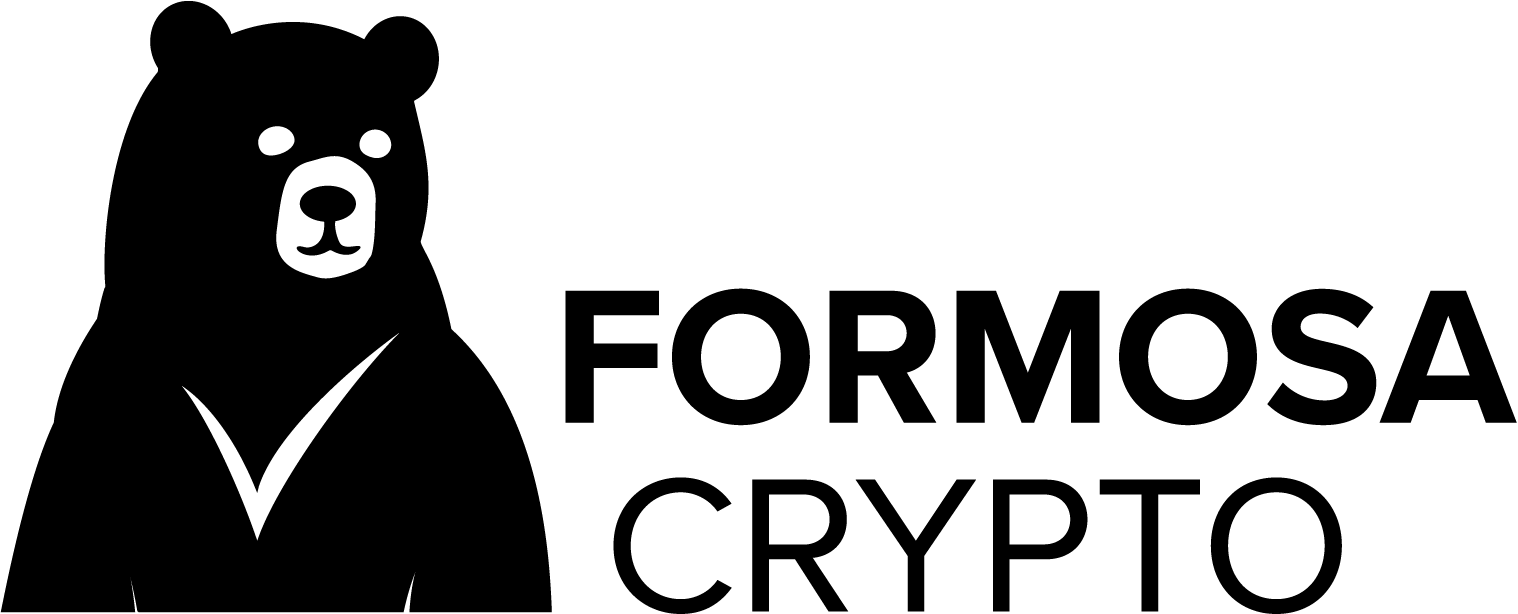
\includegraphics[width=0.4\textwidth]{formosa}
      \caption*{\Large \url{formosa-crypto.org}}
    \end{figure}
  \end{center}
  \vspace*{.5cm}
  \begin{itemize}
  \item[] \textbf{Jasmin:} \url{github.com/jasmin-lang/jasmin}
  \item[] \textbf{EasyCrypt specifications:}
    \url{github.com/formosa-crypto/crypto-specs}
  \item[] \textbf{Libjade:} \url{github.com/formosa-crypto/libjade}
  \end{itemize}
\end{frame}
